% =============================================================================
%  GELT — Gauge-Equivariant Lattice Transformer
%  Two-column PRL-style paper (revtex4-2).  Build:
%      cd paper && pdflatex gelt_paper && pdflatex gelt_paper
%  Figures are the PNGs produced by the repository's scripts, under
%  ../results/<study>/ ; \graphicspath lists those directories so bare
%  filenames keep working.
% =============================================================================
\documentclass[aps,prl,reprint,superscriptaddress,nofootinbib]{revtex4-2}

\usepackage{amsmath,amssymb,mathtools}
\usepackage{graphicx}
\usepackage{booktabs}
\usepackage{bm}
\usepackage{xcolor}
\usepackage{tikz}
\usetikzlibrary{arrows.meta,positioning,fit,backgrounds,calc}
\usepackage[colorlinks=true,linkcolor=blue!50!black,citecolor=blue!50!black,
            urlcolor=blue!50!black]{hyperref}

\graphicspath{{../}{../results/}{../results/sampler/}{../results/glueball/}
              {../results/attention/}{../results/wilson_regression/}}

% ---- shorthand --------------------------------------------------------------
\newcommand{\Tr}{\operatorname{Tr}}
\newcommand{\Obar}{\bar{O}}
\newcommand{\Abar}{\bar{A}}
\newcommand{\meff}{m_{\mathrm{eff}}}
\newcommand{\at}{a_t}
\newcommand{\as}{a_s}
\newcommand{\That}{\hat{T}}
\newcommand{\Zt}{\mathbb{Z}_2}
\newcommand{\xiA}{\xi_A}
\newcommand{\GELT}{\textsc{gelt}}

% PRL style suppresses section numbers; this paper cross-references its own
% sections, so numbering is switched back on.
\setcounter{secnumdepth}{3}

\begin{document}

\title{Gauge-Equivariant Attention for Lattice Gauge Theory:\\
Learned Variational Operators and Attention Maps as Lattice Observables}

\author{Francesco Passante}
\affiliation{Master's thesis work, lattice gauge theory and machine learning}

\date{\today}

\begin{abstract}
We introduce \GELT, a gauge-equivariant lattice transformer whose attention
scores are gauge \emph{invariant} and whose value path is matrix bilinear, with
keys and values parallel transported over the full $L^1$ ball of Manhattan
radius $R$ along an average of all shortest lattice paths. Exact invariance of
the network output is verified to machine precision. Trained on a
Rayleigh-quotient loss whose converged value \emph{is} a mass, and restricted
to a single timeslice so that the transfer-matrix bound applies, \GELT\ becomes
a variational $0^{++}$ glueball operator for $SU(2)$: on an anisotropic
$12^3\times24$, $\beta=2.4$, $\xi=3$ ensemble it saturates the variational
bound at the classical anchor $m\at\approx0.33$ and carries significantly more
ground-state weight than the optimal combination of a four-level smeared
Morningstar--Peardon basis, $\Delta A_0=+0.078\pm0.022$ ($3.6\sigma$) combining
two independently sampled ensembles, at a consistent mass. Because the
attention weights are gauge invariant, any reduction of an attention row is a
local scalar lattice operator, so the attention field itself has a mass. In
three-dimensional $\Zt$ gauge theory near criticality the correlation length
read out of the attention tracks the classical one at Pearson $0.9966$ over a
factor $2.7$ in $\xi$ and is $12\times$ more sensitive to the evaluation
ensemble than to the training coupling. Because 3D $\Zt$ is \emph{exactly} dual
to the 3D Ising model, this can be checked against ground truth rather than
against another operator: measured in the dual --- where the order parameter,
which is the non-local 't~Hooft operator on the gauge side and therefore
unavailable to any smeared-loop basis, interpolates the same mass gap with
near-unit overlap --- the trained attention field is the only arm consistent with it
($+3.8\%$) while the classical smeared basis and the untrained network read
$9\%$ and $8\%$ low. The structural statement holds already at random initialization; what
training adds is ground-state purity, $\Delta A_0=+0.11$ to $+0.27$
($5.4\sigma$--$23.5\sigma$), and it is that purity the dual confirms as
accuracy. Equivariant attention maps are therefore not diagnostics but
measurements.
\end{abstract}

\maketitle

% =============================================================================
\section{Introduction}
% =============================================================================

Lattice gauge theory turns quantum field theory into a statistical problem on a
finite grid~\cite{Wilson1974}, and the quantities it must estimate --- masses,
string tensions, topological susceptibilities --- are all expectation values of
gauge-invariant operators. Two facts make machine learning attractive here and
one makes it delicate. The first fact is that the accuracy of a lattice
measurement is usually limited not by statistics but by \emph{operator quality}:
how much of a chosen interpolating operator's spectral weight sits on the state
one wants. The second is that the search for a good operator --- choose loop
shapes, choose a smearing schedule, diagonalize a small correlator matrix --- is
an optimization problem with a differentiable objective. The delicate part is
symmetry: a network that is not gauge equivariant computes a function of the
gauge in which the configuration happens to be written, and no gauge-fixing
convention makes such a function an observable.

Lattice gauge equivariant convolutional networks (L-CNNs) resolved the symmetry
problem~\cite{Favoni2022}, by building the network out of parallel transports and
bilinear loop products so that equivariance holds exactly and by construction;
related gauge-covariant architectures followed~\cite{NagaiTomiya2021,CASK2025}.
Their convolutional kernels, however, are fixed after training: the same stencil
is applied at every site of every configuration. Attention~\cite{Vaswani2017}
removes exactly that restriction --- the aggregation weights are computed from
the content in front of the network --- but a naive attention score over gauge
fields is not an observable.

This paper develops \GELT\ (gauge-equivariant lattice transformer), which
resolves the tension with two design choices. The attention score is a
gauge-\emph{invariant} two-loop trace between a query and a parallel-transported
key, and the value path is matrix \emph{bilinear}, $\alpha\,Q_v^\dagger\tilde V$,
so that the L-CNN loop-doubling universality argument transfers directly and
each layer roughly doubles the maximum loop length the network can express.
Transport between sites is averaged over \emph{all} shortest lattice paths in
the $L^1$ ball of radius $R$, computed by a dynamic-programming recursion rather
than by enumeration, so a single block already sees a rotationally symmetric,
non-axis-aligned receptive field.

Two results follow, and they are of different kinds.

\emph{As an operator}, \GELT\ is trained without labels on the Rayleigh quotient
$C(1)/C(0)$ of the transfer matrix, whose converged value is the mass itself.
Constrained to act on a single timeslice --- the same condition that forbids
temporal smearing, applied to the network --- it becomes a legitimate
interpolating operator at every step of training, and on an anisotropic $SU(2)$
ensemble it beats a four-level smeared Morningstar--Peardon
basis~\cite{MorningstarPeardon1999} on ground-state overlap while agreeing with
it on the mass, as the variational principle demands.

\emph{As a measurement}, the attention map is an observable in its own right.
Gauge invariance of the score means any per-site reduction of an attention row
is a local gauge-invariant scalar field; single-timeslice locality means its
zero-momentum correlator has an exact spectral decomposition. The attention
field therefore has a mass, and that mass is the theory's mass gap. We verify
this in three-dimensional $\Zt$ gauge theory, where the correlation length can be
tuned over a real dynamic range, and we are careful to separate what this
establishes about the architecture from what it establishes about learning.

% =============================================================================
\section{The GELT architecture}
\label{sec:arch}
% =============================================================================

\subsection{Fields and symmetry}

Gauge fields live on links, $U_\mu(x)\in G$, and a gauge transformation is a
group element $\Omega(x)$ at every site,
\begin{equation}
  U_\mu(x)\;\longrightarrow\;\Omega(x)\,U_\mu(x)\,\Omega^\dagger(x+\hat\mu).
  \label{eq:gaugetrafo}
\end{equation}
The network's input is the untraced plaquette field
\begin{equation}
  P_{\mu\nu}(x)=U_\mu(x)U_\nu(x{+}\hat\mu)U_\mu^\dagger(x{+}\hat\nu)U_\nu^\dagger(x),
\end{equation}
one channel per plane $\mu<\nu$, which transforms in the \emph{adjoint} way,
$W(x)\to\Omega(x)W(x)\Omega^\dagger(x)$ --- the hidden state of every layer keeps
this transformation law. Color indices are carried explicitly at every stage,
even for $\Zt$ where $n_c=1$, so that every matrix product and every dagger is
written out and the implementation ports verbatim from $\Zt$ to $SU(N)$.

\subsection{Shortest-path-averaged transport}

To compare fields at $x$ and $x+\Delta x$ one must transport one to the other.
\GELT\ uses, for every signed offset in the $L^1$ ball
$1\le|\Delta x|_1\le R$, the average over \emph{all} shortest lattice paths,
\begin{equation}
  T_{\Delta x}(x)=\frac{1}{N_{\Delta x}}
  \sum_{\substack{\mathcal{P}:x\to x+\Delta x\\ |\mathcal{P}|=|\Delta x|_1}}
  U_{\mathcal{P}},
  \qquad
  N_{\Delta x}=\frac{|\Delta x|_1!}{\prod_\mu |\Delta x_\mu|!},
  \label{eq:transport}
\end{equation}
built by the recursion
\begin{equation}
\begin{split}
  T_{\Delta x}(x)=&\!\!\sum_{\mu:\Delta x_\mu>0}\!\! U_\mu(x)\,T_{\Delta x-\hat\mu}(x{+}\hat\mu)\\
  &+\!\!\sum_{\mu:\Delta x_\mu<0}\!\! U^\dagger_\mu(x{-}\hat\mu)\,T_{\Delta x+\hat\mu}(x{-}\hat\mu),
\end{split}
\end{equation}
evaluated in one pass ordered by $|\Delta x|_1$, so the cost is linear in the
number of offsets rather than in the (exponentially many) paths. Under
\eqref{eq:gaugetrafo} every term transforms identically,
$T_{\Delta x}(x)\to\Omega(x)T_{\Delta x}(x)\Omega^\dagger(x{+}\Delta x)$, so the
average is gauge covariant; unlike a single axis-aligned path it also preserves
the lattice rotation symmetry. The offset ball is the network's receptive field
per layer: $|\Delta x|_1\le R$ contains $24$ offsets in $3$D at $R=2$ and $84$
offsets in $2$D at $R=6$.

\subsection{The equivariant attention block}

One \GELT\ block (\textsc{gemhsa}, Fig.~\ref{fig:arch}) maps a covariant field
$W$ to a covariant field of the same shape:

\emph{(i) Augment and project.} The channel axis is extended by the on-site
identity and the daggers, $C\to 2C+1$, which lets a single linear map express
both a field and its inverse; four per-head projections
$Q_s,Q_v,K,V$ of width $d_{qkv}$ are then taken with complex weights shared over
sites. All four remain adjoint-covariant.

\emph{(ii) Transport.} Keys and values at $x+\Delta x$ are brought to $x$,
$\tilde K = T_{\Delta x}K T^\dagger_{\Delta x}$, so that they conjugate with
$\Omega(x)$, like the query.

\emph{(iii) Invariant score.} The score is a real trace,
\begin{equation}
  s_{x\to x+\Delta x}
  =\frac{1}{\sqrt{n_c\,d_{qkv}}}\,
  \operatorname{Re}\sum_a\Tr\!\big[\,Q_{s,a}^\dagger(x)\,\tilde K_a(x{+}\Delta x)\,\big],
  \label{eq:score}
\end{equation}
which is \emph{exactly gauge invariant}, the two $\Omega(x)$ factors cancelling
under the trace. Equation~\eqref{eq:score} is the matrix generalization of the
usual inner product $q^\dagger k$, and it is a familiar lattice object: a
two-loop correlator of the kind that measures glueball propagators and string
tensions. Relative position enters through a rotary encoding~\cite{RoPE2021}
acting on channel pairs of $K$ with an offset-dependent angle, which makes the
score offset selective without breaking invariance (it acts in channel space,
not color space).

\emph{(iv) Softmax and bilinear value path.} With
$\alpha=\mathrm{softmax}_{\Delta x}(s)$,
\begin{equation}
  W^{\rm out}(x)=\sum_{\Delta x}\alpha_{x\to x+\Delta x}\;
  Q_v^\dagger(x)\,\tilde V(x{+}\Delta x),
  \label{eq:value}
\end{equation}
a product of two covariant matrices, hence covariant. This is the key departure
from standard attention: because the value path multiplies transported loop
matrices, every layer composes longer Wilson loops, and loop degree doubles with
depth --- the mechanism behind L-CNN's universality argument~\cite{Favoni2022}.

\emph{(v) Mix, gate, residual.} A complex linear map returns the head
outputs to $C$ channels; the sublayer output is gated by a trace-activated real
scalar, $g=\mathrm{softplus}(\operatorname{Re}\Tr W_{\rm mix}/n_c)$, and added to
the untouched residual stream. A trace and a per-site MLP turn the final field
into a gauge-invariant scalar per site, i.e.\ exactly an operator density; a
spatial reduction is optional.

\begin{figure}[t]
\centering
\resizebox{\columnwidth}{!}{%
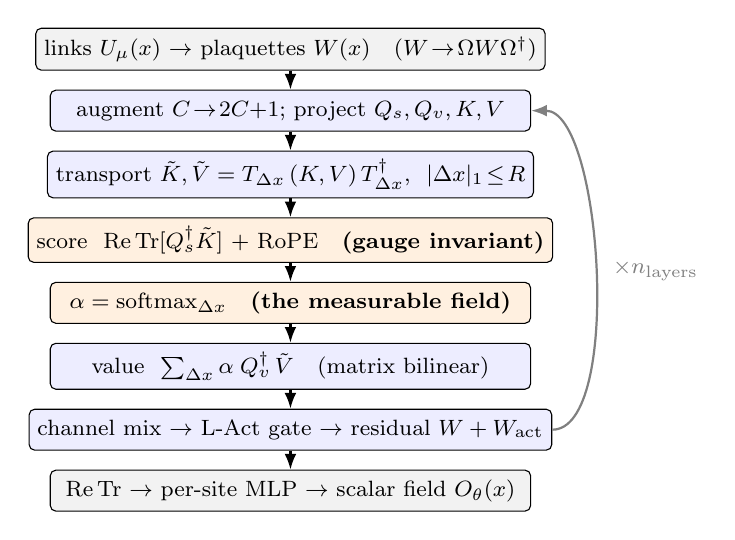
\begin{tikzpicture}[
  font=\footnotesize,
  box/.style={draw, rounded corners=2pt, align=center, inner sep=3pt,
              minimum width=6.1cm, minimum height=0.52cm},
  cov/.style={box, fill=blue!7},
  inv/.style={box, fill=orange!12},
  arr/.style={-{Latex[length=2mm]}, thick}]

\node[box, fill=gray!10] (in)  {links $U_\mu(x)$ $\to$ plaquettes $W(x)$
                                 \ \ ($W\!\to\!\Omega W\Omega^\dagger$)};
\node[cov, below=2.4mm of in] (aug) {augment $C\!\to\!2C{+}1$; project
                                 $Q_s,Q_v,K,V$};
\node[cov, below=2.4mm of aug] (tr) {transport
   $\tilde K,\tilde V=T_{\Delta x}\,(K,V)\,T^\dagger_{\Delta x}$,\ \
   $|\Delta x|_1\!\le\! R$};
\node[inv, below=2.4mm of tr] (sc) {score $\ \operatorname{Re}\Tr[Q_s^\dagger\tilde K]$
   $+$ RoPE \ \ \textbf{(gauge invariant)}};
\node[inv, below=2.4mm of sc] (sm) {$\alpha=\mathrm{softmax}_{\Delta x}$
   \ \ \textbf{(the measurable field)}};
\node[cov, below=2.4mm of sm] (val) {value $\ \sum_{\Delta x}\alpha\;
   Q_v^\dagger\,\tilde V$ \ \ (matrix bilinear)};
\node[cov, below=2.4mm of val] (mix) {channel mix $\to$ L-Act gate $\to$
   residual $W+W_{\rm act}$};
\node[box, fill=gray!10, below=2.4mm of mix] (out) {$\operatorname{Re}\Tr$
   $\to$ per-site MLP $\to$ scalar field $O_\theta(x)$};

\foreach \a/\b in {in/aug, aug/tr, tr/sc, sc/sm, sm/val, val/mix, mix/out}
  \draw[arr] (\a) -- (\b);

\draw[arr, gray] ($(mix.east)+(0,0)$) .. controls +(0.9,0) and +(0.9,0) ..
   node[right=1mm, gray]{$\times n_{\rm layers}$} ($(aug.east)+(0,0)$);
\end{tikzpicture}}
\caption{One \GELT\ block. Blue stages carry adjoint-covariant matrix fields;
orange stages are gauge singlets. The scores, and hence the attention weights
$\alpha$, are exactly gauge invariant --- which is what makes them observables
(Sec.~\ref{sec:attnop}) rather than diagnostics. The value path multiplies two
covariant matrices, so loop degree doubles with depth.}
\label{fig:arch}
\end{figure}

\subsection{Exactness of the symmetry}

Equivariance is not approximate and not learned. On random $SU(2)$
configurations with a Haar-random gauge transformation $\Omega(x)$ generated by
$QR$ decomposition, the full network output satisfies
$O_\theta[U^\Omega]=O_\theta[U]$ with a maximum drift of $0.0$ --- bit-identical
outputs --- for both positional-encoding variants in \texttt{complex128} and in
\texttt{complex64}, at $4$ layers and nonzero readout. A unit-test suite of $111$
tests covers the block equivariance
$\mathrm{block}(W^\Omega,T^\Omega)=\Omega\,\mathrm{block}(W,T)\,\Omega^\dagger$
for $SU(2)$, $SU(3)$ and $\Zt$, the covariance of the transport
\eqref{eq:transport}, and the octant identity
$T_{-\Delta x}(x)=T^\dagger_{\Delta x}(x-\Delta x)$.

\subsection{Cost}

Memory, not arithmetic, is the binding constraint: the transport tensor is
$(N_{\rm cfg}, n_{\rm off}, |\Lambda|, n_c, n_c)$ and $n_{\rm off}$ grows like
$R^D$. Two mitigations are used throughout. Restricting the network to a single
timeslice (Sec.~\ref{sec:constraint}), which the physics demands anyway,
collapses the $4$D transport to a $3$D one and cuts the cost by a factor
$\approx70$; and transports are rebuilt per batch on the fly rather than cached,
which is cheap --- the recursion \eqref{eq:transport} builds the whole $R=2$ ball
for $2000$ $8^2$ configurations in $\approx0.02$~s --- so memory is traded for a
negligible constant.

% =============================================================================
\section{Ensembles and sampling}
\label{sec:sampling}
% =============================================================================

\subsection{Actions}

All ensembles use the Wilson action
$S=\beta\sum_{x,\mu<\nu}\!\big(1-\tfrac{1}{n_c}\operatorname{Re}\Tr P_{\mu\nu}\big)$.
Spectroscopy additionally needs an \emph{anisotropic} lattice, $\at=\as/\xi$
with $\xi>1$, so that a heavy state's exponential decay is sampled by $\xi$
times more timeslices~\cite{MorningstarPeardon1999}. At tree level this is a
reweighting by plaquette orientation,
\begin{equation}
  \beta_s=\beta/\xi \ \ (\text{spatial}),\qquad
  \beta_t=\beta\,\xi \ \ (\text{temporal}),
  \label{eq:aniso}
\end{equation}
which we fold into the staple sum so that $\xi=1$ reproduces the isotropic code
path bit for bit.

\subsection{Exact local updates}

$SU(2)$ admits two exact, tuning-free local updates whose combination beats
Metropolis critical slowing down. The heat
bath~\cite{Creutz1980,KennedyPendleton1985} exploits the fact that a sum of
$SU(2)$ elements is proportional to an $SU(2)$ element, $A=kV$, so the
single-link conditional distribution is known in closed form and the new link is
independent of the old. Overrelaxation~\cite{Creutz1987} reflects
$U\to V^\dagger U^\dagger V^\dagger$, preserving the action exactly while moving
as far as possible across the constant-action surface; since the reflection is
expansive off the group manifold, each link is re-projected onto $SU(2)$ in
closed form. The production sweep is one heat-bath sweep followed by
$n_{\rm OR}=4$ overrelaxation sweeps in a checkerboard pattern.

For $\Zt$ the analogous exact update is $P(U=+1)=\sigma(2\beta s)$ with $s$ the
staple sum. It is not a convenience but a necessity near criticality: the
single-link Metropolis proposal is the flip $U\to-U$, whose acceptance collapses
to $\approx0.02$ as the configuration orders, freezing the chain exactly where
the correlation length is largest.

\subsection{Validation and autocorrelation}

Figure~\ref{fig:sampler} shows the standard checks for $SU(2)$: thermalization,
the exactly known two-dimensional mean plaquette $I_2(\beta)/I_1(\beta)$
reproduced across three volumes, the three-dimensional confining crossover, and
the plaquette autocorrelation ($\tau_{\rm int}\approx4.5$ sweeps for Metropolis
at $\beta=0.8$). The anisotropic action is validated separately
(Fig.~\ref{fig:aniso}): at $\xi=1$ it returns the exact two-dimensional
plaquette, $0.4329\pm0.0017$ against $0.4331$ ($0.1\sigma$); at $\xi>1$ the
plaquette splits in the intended direction, $\langle P_{st}\rangle$ rising and
$\langle P_{ss}\rangle$ falling; and a Creutz-ratio estimate gives a
\emph{renormalized} anisotropy $\xi_R\approx3.32$ at bare $\xi=3$ --- the
expected tree-level mismatch, measured rather than tuned away.

Configurations are separated by $n_{\rm skip}$ sweeps set from the integrated
autocorrelation time of the \emph{measured} observable (Madras--Sokal
windowing~\cite{MadrasSokal1988}), not of the plaquette: extended operators
decorrelate more slowly. For the anisotropic $SU(2)$ ensembles the smeared
glueball operator gives $\tau_{\rm int}\approx2$ and we take $n_{\rm skip}=5$;
for $\Zt$ near $\beta_c$ critical slowing down ($\tau\sim\xi^z$, $z\approx2$)
gives $\tau_{\rm int}\approx44$ sweeps and we take $n_{\rm skip}=200$. Errors
are always jackknife, blocked when residual autocorrelation is suspected, and
comparisons between two operators measured on the same configurations are
always jackknifed as a \emph{difference}, so that the shared ensemble
fluctuations cancel.

Table~\ref{tab:ensembles} lists every ensemble used below.

\begin{figure*}[t]
\centering
\includegraphics[width=0.92\textwidth]{sampler_validation_su2_metropolis.png}
\caption{$SU(2)$ Monte Carlo validation. Top left: thermalization of the mean
plaquette at four couplings against the exact $I_2(\beta)/I_1(\beta)$ (dashed).
Top right: the two-dimensional mean plaquette reproduces the exact curve at
$L=4,8,16$. Bottom left: the three-dimensional confining crossover, with the
strong-coupling $\beta/4$ asymptote. Bottom right: plaquette autocorrelation,
$\tau_{\rm int}\approx4.5$ sweeps. The equivalent four-panel check for $\Zt$
reproduces $\langle P\rangle=\tanh\beta$ in two dimensions and the transition
near $\beta_c\approx0.761$ in three.}
\label{fig:sampler}
\end{figure*}

\begin{figure*}[t]
\centering
\includegraphics[width=0.74\textwidth]{anisotropy_validation.png}
\caption{The anisotropic action. Left: at $\xi=1$ the anisotropic code path
reproduces the exact two-dimensional $SU(2)$ plaquette to $0.1\sigma$. Right: at
$\xi>1$ temporal plaquettes grow and spatial ones shrink, as
Eq.~\eqref{eq:aniso} requires; a Creutz-ratio estimate returns
$\xi_R\approx3.32$ at bare $\xi=3$.}
\label{fig:aniso}
\end{figure*}

\begin{table}[t]
\caption{Ensembles. All errors quoted in this paper are jackknife estimates over
configurations, blocked where indicated.}
\label{tab:ensembles}
\begin{ruledtabular}
\footnotesize
\begin{tabular}{lcccl}
theory & lattice & coupling & $N$ & use \\
\colrule
$SU(2)$, 4D & $12^3{\times}24$ & $\beta{=}2.4$, $\xi{=}3$ & 2000
  & anchor $+$ training \\
$SU(2)$, 4D & $12^3{\times}24$ & $\beta{=}2.4$, $\xi{=}3$ & 2000
  & replication \\
$SU(2)$, 4D & $12^3{\times}24$ & $\beta{=}2.4$, $\xi{=}3$ & 32
  & attention readout \\
$SU(2)$, 4D & $12^3{\times}24$ & $\beta{\in}[2.1,2.7]$ & 2000
  & $\xi_s$ scan \\
$\Zt$, 3D & $24^2{\times}48$ & $\beta{\in}[0.745,0.76]$ & 2000
  & attention operator \\
$SU(2)/\Zt$, 2D & $8^2$ & $\beta{=}2.4/0.7$ & 2000
  & regression \\
\end{tabular}
\end{ruledtabular}
\vspace{-2mm}
\begin{flushleft}\footnotesize
$SU(2)$: heat bath $+\,4$ overrelaxation sweeps, $n_{\rm skip}=5$.
$\Zt$: exact heat bath, $n_{\rm skip}=200$. 2D regression sets: Metropolis.
\end{flushleft}
\end{table}

% =============================================================================
\section{Supervised benchmarks}
\label{sec:regression}
% =============================================================================

Before using \GELT\ as an operator we check what it can represent, on targets
whose answer is known exactly.

\paragraph{The inductive-bias gap.} The motivating observation is that a
non-equivariant convolutional network fed \emph{links} cannot learn the Wilson
action ($R^2\approx0$ across volumes on Haar-random $\Zt$ data), because the
target requires multiplying four specific link matrices around a plaquette --- a
product an additive kernel does not express --- while the same network fed
\emph{plaquettes} reaches $R^2\approx0.99$, the task having collapsed to a linear
sum. The gap is precisely what an equivariant transport supplies. (On Haar data
even a perfect regressor only memorizes the action \emph{function}; the
$\beta$-dependent physics below requires the Monte Carlo data path of
Sec.~\ref{sec:sampling}.)

\paragraph{An exactly representable target.} The naive topological charge
density $q(x)$ is a single matrix bilinear in the plaquettes at $x$. \GELT's
value path \eqref{eq:value} is matrix bilinear, so the target lies inside the
hypothesis class algebraically. A $10\,673$-parameter model ($20\,241$ real
degrees of freedom) at $L=8$, $D=4$, $\beta=2.4$, $R=2$ reaches
$R^2=1.0000$ on held-out $SU(2)$ configurations, with the training loss reaching
the float32 floor. This is a representation check rather than a learning result,
and its lesson is stated as such: a target that needs no context is fit with no
context.

\paragraph{Receptive field and transport mode.} Rectangular $R\times T$ Wilson
loops probe the opposite regime, where the target's support exceeds one block's
reach. Table~\ref{tab:transport} scans loop size against the two transport modes
of Eq.~\eqref{eq:transport} at fixed $R=2$, in both gauge groups. The pattern is
unambiguous and is about geometry, not about paths: the $1\times1$ loop is fit
exactly, the $2\times2$ loop --- whose extent already matches the ball --- is
fit well, and the $3\times3$ loop, which no depth-limited $R=2$ stack can close,
is not fit at all. Between the shortest-path average and a single canonical path
there is no consistent difference: the average is ahead by $0.07$ and $0.04$ in
$R^2$ on $\Zt$ and behind by $0.01$ on $SU(2)$, i.e.\ within run-to-run scatter.
Path averaging is therefore adopted for its symmetry --- it preserves lattice
rotation invariance, which a canonical path breaks --- and not for accuracy;
projecting the averaged transport back onto the group, a third variant, costs a
transport build of $2.9$~s and buys nothing.

\begin{table}[t]
\caption{Test $R^2$ for per-site $R\times T$ Wilson-loop regression at fixed
receptive radius $R=2$ on $8^2$ lattices, $N=2000$ configurations, $40$ epochs.
``avg'' is the shortest-path average of Eq.~\eqref{eq:transport}, ``single'' one
canonical shortest path, ``proj'' the average projected back onto the group.
Accuracy is governed by the receptive radius, not by the transport mode.}
\label{tab:transport}
\begin{ruledtabular}
\begin{tabular}{lccccc}
 & \multicolumn{2}{c}{$\Zt$, $\beta=0.7$} & \multicolumn{3}{c}{$SU(2)$, $\beta=2.4$}\\
\cline{2-3}\cline{4-6}
loop & avg & single & avg & single & proj \\
\colrule
$1\times1$ & $0.99999$ & $0.99999$ & $1.000$ & $1.000$ & $1.000$ \\
$2\times2$ & $0.871$ & $0.799$ & $0.979$ & $0.988$ & $0.972$ \\
$3\times3$ & $0.299$ & $0.259$ & $0.022$ & $-0.005$ & $-0.004$ \\
\end{tabular}
\end{ruledtabular}
\end{table}

% =============================================================================
\section{A network as a variational operator}
\label{sec:spectroscopy}
% =============================================================================

\subsection{Masses, and why glueballs are hard}

With periodic temporal extent $N_t$ and transfer matrix
$\That=e^{-\at\hat H}$~\cite{OsterwalderSeiler1978}, the connected correlator of
a zero-momentum operator $\Obar(t)=\sum_{\vec x}O(\vec x,t)$ decomposes as
\begin{equation}
  C(\Delta)=\big\langle\delta\Obar(t{+}\Delta)\,\delta\Obar(t)\big\rangle
  =\sum_{n>0}\big|\langle0|\hat{\bar O}|n\rangle\big|^2 e^{-m_n\Delta\at}+\dots,
  \label{eq:spectral}
\end{equation}
the ellipsis being the periodic image. Every term is positive, so
$\meff(\Delta)=\log[C(\Delta)/C(\Delta{+}1)]$ approaches the ground-state mass
\emph{from above}: the correlator is a variational bound machine. The $0^{++}$
glueball is the hard case~\cite{Berg1980}: its variance is itself a vacuum-channel
correlator, so noise is $\Delta$-independent while signal decays, giving
${\rm S/N}\sim\sqrt{N}e^{-m_G\Delta\at}$~\cite{Lepage1989}. Since $m_G a$ is of
order one, the signal is gone within a few slices and more statistics barely
help. The plateau must instead be dragged to \emph{small} $\Delta$, which means
building an operator whose spectral weight already sits on the ground state ---
the entire craft of glueball spectroscopy, classically executed with APE
smearing~\cite{APE1987} and a generalized eigenvalue problem
(GEVP)~\cite{MichaelTeasdale1983,LuscherWolff1990,Blossier2009,MorningstarPeardon1999}
over a basis of smearing levels.

\subsection{The Rayleigh loss}

Let $O_\theta$ be any gauge-invariant scalar field built from the spatial links
of timeslice $t$, and $|\psi\rangle=(\hat{\bar O}_\theta-\langle\Obar_\theta\rangle)|0\rangle$.
Then $C(\Delta)=\langle\psi|\That^\Delta|\psi\rangle$ with
$\langle\psi|0\rangle=0$, so
\begin{equation}
  R(\theta)=\frac{C(1)}{C(0)}
  =\frac{\langle\psi|\That|\psi\rangle}{\langle\psi|\psi\rangle}\;\le\;e^{-m_G\at},
  \label{eq:rayleigh}
\end{equation}
a Rayleigh quotient of the transfer matrix restricted to the non-vacuum sector.
Training on $\mathcal{L}=-C(1)/C(0)$ is therefore variational: no labels, no
supervision, the training signal is the same Monte Carlo correlator the
classical analysis measures, the bound holds at every step because equivariance
makes $O_\theta$ a legitimate operator for \emph{any} $\theta$, and at
convergence $m_G\at=-\log R$ --- the converged loss \emph{is} the mass. In
practice we average two ratios,
$\mathcal{L}=-\frac12[C(1)/C(0)+C(2)/C(0)]$, whose floor at $m\at=0.33$ is
$\approx-0.62$.

\subsection{The single-timeslice constraint}
\label{sec:constraint}

Equation~\eqref{eq:rayleigh} required $\Obar(t)$ to depend on timeslice $t$
alone --- the same condition that forbids smearing in time. A four-dimensional
network violates it twice, through temporal plaquettes in its input and through
a receptive field that leaks across slices, and the violation is not a small
correction: it makes the loss \emph{gameable}. If $O(t)$ may depend on
neighboring slices, the cheapest route to $C(1)/C(0)\to1$ is an output that
varies slowly in $t$; in the limit a per-configuration constant gives a fake
mass of zero. We therefore run \GELT\ as a \emph{three-dimensional} network on
the spatial links of one timeslice, batched over
(configuration $\times$ timeslice). Within its slice the operator keeps its full
spatial loop-building power, which is exactly the domain the classical operator
uses. The constraint that protects the physics also pays the memory bill
(Sec.~\ref{sec:arch}).

\subsection{Making the loss trainable}

Three pathologies had to be removed, each of which is a property of the
objective rather than of the architecture.
(i) \emph{Zero gradient at initialization}: $C(0)$ and $C(1)$ are both quadratic
in the output, so a zero-initialized readout --- a common stabilization --- sits
at an exact saddle and training never starts; the readout must be initialized
nonzero.
(ii) \emph{Denominators}: chaining ratios $C(\Delta)/C(\Delta{-}1)$ places the
small, signed, noisy $C(1)$ in a denominator, which keeps values finite but
makes gradients meaningless; every ratio uses the large positive $C(0)$, and the
correlator arithmetic runs in float64.
(iii) \emph{The scale-flat direction}: the quotient is invariant under
$O\to\lambda O$, an exactly flat direction along which the bilinear value path's
squared per-layer gain drives $C(0)$ to float32 overflow once the inputs are
smooth. Adding $10^{-2}(\log C(0))^2$ pins the scale without touching the ratio,
hence without biasing the physics.
Finally, the bound holds in expectation and not on a finite sample, so all
reported numbers come from a hard split (70/10/20, contiguous in Monte Carlo
time) with checkpoint selection on validation and blocked jackknife on the
untouched test configurations.

\subsection{The classical anchor}

The classical measurement (Fig.~\ref{fig:classical}) is the orientation-summed
spatial Wilson loop at APE levels $0,2,4,6$, analyzed with the connected
correlator, $\meff$, and a GEVP at $t_0=1$. On the isotropic $12^4$ lattice
there is no plateau at all --- the signal dies by $\Delta\approx3$ and no
operator basis can repair a lattice --- while on the anisotropic
$12^3\times24$, $\xi=3$ ensemble $C(\Delta)$ decays cleanly over $10$--$12$
slices and the GEVP ground state gives
\begin{equation}
  \meff(1)=0.365\pm0.008,\quad \meff(2)=0.333\pm0.011,
\end{equation}
confirmed at $\meff(3)=0.333\pm0.036$ on the held-out split, i.e.\ an anchor
$m\at\approx0.33$. We stress what this number is not: with $\beta_s=\beta/\xi=0.8$
the spatial lattice is coarse, so $m\as=\xi\,m\at\approx1.0$ is not continuum
physics. The claim established is that a plateau exists on this ensemble, which
is what the learned operator must be judged against.

\begin{figure*}[t]
\centering
\includegraphics[width=0.92\textwidth]{glueball_validation.png}
\caption{Classical $0^{++}$ baseline on the anisotropic ensemble
($12^3\times24$, $\beta=2.4$, $\xi=3$, $N=2000$). Top left: the analysis chain
recovers a known mass from a synthetic single-exponential correlator. Top right:
smearing monotonicity. Bottom left: the connected correlator decays over
$10$--$12$ slices, symmetric about $\Delta=N_t/2$. Bottom right: effective
masses; the multi-level GEVP ground state (green) plateaus near $0.33$ where the
single operators do not, and stays resolved where the thin operator's errors
explode.}
\label{fig:classical}
\end{figure*}

\subsection{Result: a learned operator that wins on overlap}

Fed \emph{thin} plaquettes, the learned operator is genuine but loses: its
$\meff$ descends $0.705\to0.527\to0.441\to0.310$ and it far outperforms the thin
classical operator, but it sits above the smeared GEVP at small $\Delta$ and,
appended to the classical basis as a fifth operator, changes the GEVP by
fractions of an error bar. The diagnosis is a depth budget --- four bilinear
layers compose loops of degree $\le16$, while six APE steps contain branched
staple content of degree $\sim3^6$ within the same radius --- and the
correlation of the learned operator with the smearing ladder peaks at APE$\times2$
($|r|=0.68,\mathbf{0.87},0.71,0.59$ for levels $0,2,4,6$): the network relearned
about two smearing steps.

The fix is to supply the smearing and let the network do what smearing cannot.
Feeding plaquettes built at the same cumulative APE levels the GEVP uses
($0,2,4,6$; $3$ planes $\times$ $4$ levels $=12$ input channels), with transport
still built from thin links, makes the comparison maximally sharp: both methods
see \emph{exactly} the same smearing levels, the GEVP may take one global linear
combination of them, and the network may mix them nonlinearly and site by site.
Any gap is then attributable to the network. Training is stable with the scale
pin and reaches a best validation loss of $-0.6185$, i.e.
\begin{equation}
  m\at\approx0.329:
\end{equation}
the Rayleigh quotient \emph{saturates the transfer-matrix bound at the anchor
mass}. Table~\ref{tab:meff} and Fig.~\ref{fig:run5} give the test-split
comparison.

\begin{table}[t]
\caption{Test effective masses in units of $\at$, blocked jackknife on the $400$
held-out configurations. The learned operator plateaus from $\Delta=1$; the
enlarged five-operator GEVP collapses onto it.}
\label{tab:meff}
\begin{ruledtabular}
\begin{tabular}{lcccc}
operator & $\meff(1)$ & $\meff(2)$ & $\meff(3)$ & $\meff(4)$\\
\colrule
\GELT\ (learned) & $\bm{0.370(16)}$ & $\bm{0.333(20)}$ & $0.345(29)$ & --- \\
classical GEVP & $0.398(16)$ & $0.357(25)$ & $0.333(36)$ & $0.284(50)$ \\
GEVP $+$ \GELT & $0.366(17)$ & $0.333(20)$ & $0.347(30)$ & $0.319(48)$ \\
\end{tabular}
\end{ruledtabular}
\end{table}

Because both operators are measured on the same configurations their errors are
correlated, and the honest test is a blocked jackknife of the \emph{difference}:
\begin{equation}
  \Delta\meff\big|_{\Delta=1}=-0.028\pm0.007\ (3.9\sigma),
\end{equation}
with $-0.024\pm0.014$ at $\Delta=2$ and $+0.012\pm0.021$ at $\Delta=3$. The
learned operator sits significantly below the classical GEVP exactly where
excited-state contamination lives, and is statistically identical on the plateau
--- a better operator measuring the same physics, which is what the variational
principle demands of a legitimate win. Two corroborating facts: offered the
four-level ladder \emph{plus} \GELT, the variational solver picks essentially
pure \GELT\ (the enlarged basis matches \GELT's own $\meff$ to $\sim0.004$ at
$\Delta=1$); and the ladder-independent part of the learned operator's variance
\emph{grew} from $\sim8\%$ to $\sim18\%$ during training while the loss improved,
so the win is driven by the network's own content and not by residual noise.

\begin{figure*}[t]
\centering
\includegraphics[width=0.92\textwidth]{glueball_gelt_GELT_beats_GEVP.png}
\caption{The learned variational operator. Left: Rayleigh training curves; the
validation loss sits on the variational floor,
$-0.6185\leftrightarrow m\at\approx0.329$ (validation below training is an
estimator artifact --- the $6$-configuration batch estimator is noise-biased
toward zero while the $200$-configuration validation estimate is cleaner).
Right: test effective masses. The learned operator (green) is flat on the anchor
(dashed) from $\Delta=1$, below the still-descending classical GEVP (red) at
small $\Delta$; the enlarged GEVP${+}$\GELT\ basis (purple) collapses onto pure
\GELT.}
\label{fig:run5}
\end{figure*}

\subsection{Quoting the result: cosh fits and the overlap $A_0$}

Effective masses are how lattice results are \emph{plotted}; masses are
\emph{quoted} from a fit, and operator quality --- what this comparison is
actually about --- is quoted as the ground-state overlap, the number
Morningstar and Peardon use to rank smeared operators~\cite{MorningstarPeardon1999}.
We fit each connected correlator to the periodic single-state form
\begin{equation}
  C(\Delta)\approx A\big[e^{-m\at\Delta}+e^{-m\at(N_t-\Delta)}\big]
  \label{eq:cosh}
\end{equation}
over one \emph{shared} window $\Delta\in[2,7]$ --- comparability beats
per-operator optimality, and starting at $\Delta=2$ keeps the GEVP's residual
$\Delta=1$ contamination out of its own mass fit, since that contamination is
what the overlap should report. Extrapolating the fitted ground state back to
$\Delta=0$ gives
\begin{equation}
  A_0=\frac{A\big(1+e^{-m\at N_t}\big)}{C(0)}\in(0,1],
  \label{eq:A0}
\end{equation}
the fraction of the operator's spectral weight carried by the glueball. This
closes a conceptual loop: the Rayleigh quotient is, up to the wrap term, a
weighted average $\sum_n w_n e^{-m_n\at}$ with $w_{\rm ground}=A_0$, so
saturating the variational bound \emph{is} the statement $A_0\to1$. Objective
and metric coincide.

The right comparator for a single learned operator is not a whole basis but the
best single operator that basis contains, which the GEVP supplies: the
ground-state eigenvector $v_0$ at $(t_0,t_d)=(1,2)$ defines the fixed-vector
\emph{projected} operator $\sum_i(v_0)_i\Obar_i$~\cite{Blossier2009}. The entire
fit, $v_0$ included, is redone inside each delete-block jackknife sample.
Table~\ref{tab:overlap} and Fig.~\ref{fig:overlap} give the result, with the
correlated differences
\begin{equation}
  \Delta(m\at)=-0.008\pm0.014,\quad
  \Delta A_0=+0.066\pm0.031\,(2.1\sigma).
\end{equation}
In the field's own language: \emph{both operators measure the same mass, but the
learned operator carries $90\%$ of its spectral weight on the ground state
against $84\%$ for the optimal combination of the entire classical basis.} Note
also that the GEVP gains only $\sim0.03$ of overlap over its best single member,
while one learned operator gains $\sim0.10$ over the whole basis.

\begin{table}[t]
\caption{Cosh fits \eqref{eq:cosh} on the shared window $\Delta\in[2,7]$,
blocked jackknife on $400$ held-out configurations, for the primary ensemble and
for an independently sampled replication ensemble. $\chi^2/\mathrm{dof}$ is
artificially low because neighboring $C(\Delta)$ are strongly correlated while
the $\chi^2$ is diagonal; it is a fit-quality heuristic, and the quoted errors
come from the jackknife, which propagates the correlations correctly.}
\label{tab:overlap}
\begin{ruledtabular}
\begin{tabular}{llccc}
ensemble & operator & $m\at$ & $A_0$ & $\chi^2/\mathrm{dof}$\\
\colrule
primary & \GELT\ (learned) & $0.332(27)$ & $\bm{0.903(47)}$ & $0.05$\\
        & GEVP-projected   & $0.340(30)$ & $0.837(56)$ & $0.04$\\
        & APE$\times6$     & $0.340(32)$ & $0.805(52)$ & $0.11$\\
\colrule
replication & \GELT\ (learned) & $0.374(31)$ & $\bm{1.013(62)}$ & $0.01$\\
            & GEVP-projected   & $0.400(38)$ & $0.925(71)$ & $0.08$\\
            & APE$\times6$     & $0.390(37)$ & $0.901(68)$ & $0.05$\\
\end{tabular}
\end{ruledtabular}
\end{table}

\begin{figure*}[t]
\centering
\includegraphics[width=0.92\textwidth]{glueball_overlap_run5.png}
\caption{The result in standard spectroscopic form. Left: test $\meff(\Delta)$
for \GELT\ (green) and the projected GEVP operator (red) with their fitted-mass
bands over the shared window; the quoted mass is the band, not any single point,
and both sit on the classical anchor (dashed). Right: the ground-state fraction
$\rho(\Delta)=[C(\Delta)/C(0)]/\cosh_{\rm ref}(\Delta)$, flat at $A_0$ for a pure
interpolator; the excess at small $\Delta$ is excited-state contamination. Thin
links collapse to $\rho\approx0.25$ immediately, the classical operators descend
through $\Delta\approx3$ toward $A_0\approx0.80$--$0.84$, and \GELT\ is flat at
$A_0\approx0.90$ from $\Delta=1$.}
\label{fig:overlap}
\end{figure*}

\subsection{Replication on an independent ensemble}

The entire chain --- sampling, from-scratch training, checkpoint selection,
test-split analysis --- was repeated with a different sampler seed, nothing
tuned on the new data. The operator-quality result reproduces
(Table~\ref{tab:overlap}, Fig.~\ref{fig:replication}):
$\Delta A_0=+0.089\pm0.030$ ($2.9\sigma$), with a correlated $\meff$ difference
of $-0.038\pm0.008$ ($4.5\sigma$) at $\Delta=1$ --- the same pattern, if
anything stronger. The two independent ensembles combine to
\begin{equation}
  \Delta A_0^{\rm comb}=+0.078\pm0.022\qquad(3.6\sigma).
  \label{eq:combined}
\end{equation}

What does \emph{not} replicate is equally instructive. On the new ensemble every
operator, classical and learned alike, reads $\sim1\sigma$ heavier, and training
converged to a best Rayleigh loss of $-0.564$, decoding to $m\approx0.395$ ---
saturated to $\sim0.004$, exactly as before, but of a different floor. The
Rayleigh floor is the variational bound \emph{as realized on the sampled data},
an empirical property of the ensemble: loss values do not replicate between
independent ensembles, operator-quality statements do.

\begin{figure*}[t]
\centering
\includegraphics[width=0.92\textwidth]{glueball_overlap_ens1.png}
\caption{Figure~\ref{fig:overlap} repeated on the independently sampled
replication ensemble. The overall mass scale sits $\sim1\sigma$ higher --- both
operators agree on that shift, as they must --- while the operator-quality
ordering is unchanged: \GELT\ flat at its $A_0$ from small $\Delta$, the
classical operators descending into it.}
\label{fig:replication}
\end{figure*}

% =============================================================================
\section{The attention map as a lattice operator}
\label{sec:attnop}
% =============================================================================

\subsection{The claim}

The attention weights $\alpha_{x\to x+\Delta x}$ are computed from the invariant
score \eqref{eq:score}, so they are gauge invariant at every site. Therefore
\emph{any} reduction of an attention row to a scalar,
\begin{equation}
  A(x)=f\big(\alpha_{x\to\cdot}\big),
  \label{eq:reduction}
\end{equation}
is a local gauge-invariant scalar field built from the links --- an ordinary
lattice operator. We use three qualitatively different reductions: the self
weight $\alpha_{x\to x}$, the radial first moment
$\sum_{\Delta x}|\Delta x|_1\alpha$, and the offset entropy
$-\sum\alpha\log\alpha$. Since the trained operator is per timeslice
(Sec.~\ref{sec:constraint}), $A(t,\vec x)$ depends on slice $t$ alone, its
zero-momentum sum $\Abar(t)$ is a legitimate timeslice operator, and
Eq.~\eqref{eq:spectral} applies verbatim:
\begin{equation}
  \boxed{\ \xiA=1/m_A \overset{?}{=} \xi(\beta)\ }
\end{equation}
with no ceiling and no geometric offset, because the correlator correlates a
zero-mean \emph{fluctuation} rather than a moment of a kernel. Three
consequences, in increasing order of interest: $\xiA$ should track $\xi(\beta)$;
this measurement \emph{does not exist for a convolution}, whose kernel is fixed
so that $\delta A\equiv0$ and $C_A\equiv0$ identically; and the overlap $A_0$ of
the attention field says whether \emph{training} taught the routing to look at
the physics or whether the equivariant construction alone is responsible.

That last distinction is essential, because the first consequence is close to a
theorem --- any local gauge-invariant scalar has a correlator decaying at the
mass gap, a randomly initialized network's attention field included. The design
therefore has three arms: a trained network on its own ensemble; each trained
network on \emph{all} ensembles (so that operator quality is a property of the
row and physics a property of the column); and a random-initialization control.

\subsection{Testbed and protocol}

The measurement needs a correlation length that is large compared with one
lattice spacing and tunable over a real range. The anisotropic $SU(2)$ ensembles
of Sec.~\ref{sec:spectroscopy} supply neither: a classical GEVP scan gives
spatial correlation lengths $\xi_s=1/(\xi\,m\at)$ of
$0.57,0.83,1.00,1.10,1.00$ at $\beta=2.1,2.3,2.4,2.5,2.7$ --- never more than
$1.1$ spacings, so the whole object fits inside one grid cell. (The box is
large, $L/\xi_s\approx12$; it is the spacing that is coarse, because
$\beta_s=\beta/\xi\approx0.8$ is strong coupling.) Three-dimensional $\Zt$ gauge
theory~\cite{Wegner1971} does supply both: it is dual to the 3D Ising model, has
a second-order point at $\beta_c=0.7614133$ (the image under the duality of the
Ising $\beta^\ast_c=0.221654626(5)$~\cite{FerrenbergXuLandau2018}), and gives
$\xi=2.1\to6.4$ over four ensembles at $24^2\times48$, $N=2000$. The price is
that the conclusion is a statement about the method, not about $SU(N)$.

A fifth ensemble at $\beta=0.7600$ was measured and is \emph{excluded}. The dual
determination of Sec.~\ref{sec:dual} puts its true $\xi$ at $\approx10$ against
$L=24$, so every operator there --- classical, trained and random alike --- is
measuring the box and reads $50$--$58\%$ low. It cannot discriminate between
operators and is dropped, together with the network trained on it. Excluding it
costs no dynamic range, since $\beta=0.7585$ already carries the largest
correlation length the volume can hold. We note that the original
finite-volume guard, $\xi\le L/4$, admitted this point because it was evaluated
against the \emph{classical} $\xi\approx4.7$ --- a contaminated underestimate of
the very quantity being bounded. A finite-volume cut has to be applied to an
uncontaminated $\xi$, which is one more thing the dual supplies.

One variational operator per $\beta$ was trained exactly as in
Sec.~\ref{sec:spectroscopy} --- per-timeslice (2D here), $R=6$, four layers, two
heads, four cumulative APE input levels $(0,4,8,16)$, Rayleigh loss --- on
\texttt{configs[:800]}; \emph{all} measurements below use \texttt{configs[800:]},
so the evaluation set is unseen by every checkpoint, the diagonal included. Per
(network, ensemble) pair and for each of the $4\times2\times3=24$ attention
channels we stash $\alpha$ under \texttt{no\_grad}, reduce it by
Eq.~\eqref{eq:reduction}, form $\Abar(t)$, project the channel basis onto its
GEVP ground vector with a variational self-check (fall back to the best single
channel whenever the projection interpolates worse than a basis member), fit
Eq.~\eqref{eq:cosh} over $\Delta\in[2,8]$, and take errors from a blocked
jackknife with block $20$. The classical smeared basis is re-measured on the
\emph{same} configurations so that differences are correlated. Two nulls are
used: a config-scramble, in which each timeslice is drawn from an independently
permuted configuration, which destroys both the temporal correlation and the
per-configuration zero mode; and a time-shuffle, which is \emph{not} a null but a
zero-mode consistency check, since permuting timeslices preserves each
configuration's mean and leaves a flat pedestal $(2\xi-1)/N_t$.

\subsection{Results}

Table~\ref{tab:z2} is the diagonal run on $1200$ unseen configurations per
ensemble.
\begin{equation}
  \mathrm{Pearson}(\xiA,\xi_{\rm class})=\bm{0.9966},\qquad\text{slope }1.21,
\end{equation}
over a factor $2.74$ of classical dynamic range at $5$--$7\%$ precision on both
sides. At $\beta=0.7585$, the ensemble with the largest correlation length the
volume can hold, the normalized correlator profiles read
\begin{center}\footnotesize
\begin{tabular}{@{}lcccc@{}}
\toprule
$C(\Delta)/C(0)$ & $\Delta=1$ & 2 & 3 & 4\\
\midrule
classical basis & $0.441$ & $0.303$ & $0.230$ & $0.192$\\
trained attention & $\bm{0.695}$ & $\bm{0.565}$ & $\bm{0.477}$ & $\bm{0.406}$\\
random attention & $0.508$ & $0.351$ & $0.271$ & $0.223$\\
time-shuffle & $0.236$ & $0.229$ & $0.231$ & $0.234$\\
\bottomrule
\end{tabular}
\end{center}
--- the trained attention field is a visibly cleaner exponential than either the
classical basis or the untrained network. The last row is the zero-mode
consistency check rather than a null: permuting timeslices destroys the
temporal correlation but preserves each configuration's mean, leaving the flat
pedestal $(2\xiA-1)/N_t\approx0.26$ that is observed. The actual null is the
config-scramble, which is flat at the $10^{-2}$ level with no fittable mass (in
the full cross matrix, $26$ of $30$ null cells do not fit at all and the
remaining four return $|A_0|\le0.0066$).

\begin{table}[t]
\caption{Correlation lengths and ground-state overlaps of the attention field on
$1200$ unseen configurations per ensemble, against the classical smeared basis
measured on the same configurations and against a randomly initialized network
of identical architecture. $\Delta A_0$ is a blocked jackknife of the trained
$-$ random \emph{difference} on shared configurations; $\delta A/A$ is the
site-level fluctuation-to-mean ratio, median over the $24$ channels.}
\label{tab:z2}
\begin{ruledtabular}
\scriptsize
\setlength{\tabcolsep}{2.6pt}
\begin{tabular}{lccccc}
$\beta$ & $\xi_{\rm class}$ & $\xiA$ trained & $\xiA$ random
        & $A_0$ tr./rnd./cl. & $\Delta A_0$ \\
\colrule
$0.7450$ & $2.04(14)$ & $2.24(12)$ & $2.08(13)$ & $0.85/0.70/0.58$
  & $+0.144(17)$ \\
$0.7520$ & $2.34(16)$ & $2.76(13)$ & $2.46(16)$ & $0.78/0.67/0.58$
  & $+0.110(20)$ \\
$0.7560$ & $4.08(27)$ & $4.48(30)$ & $4.08(26)$ & $0.74/0.53/0.45$
  & $+0.204(12)$ \\
$0.7585$ & $5.59(34)$ & $6.64(32)$ & $5.47(31)$ & $0.75/0.49/0.41$
  & $+0.267(11)$ \\
\end{tabular}
\end{ruledtabular}
\end{table}

\paragraph{No memorization.} Table~\ref{tab:cross} evaluates all four networks
on all four ensembles. The matrix reads across, not down:
\begin{equation}
  \frac{\text{spread within a row (evaluation)}}
       {\text{spread within a column (training }\beta)}
  =\frac{1.477}{0.123}=\bm{12.0},
\end{equation}
and the column means correlate with the classical $\xi$ at Pearson $0.9992$. The
mean diagonal advantage in $A_0$ is only $+0.038$ and is inconsistent in sign,
against a mean trained-minus-random of $+0.156$: the learning effect is
$4\times$ the $\beta$-matching effect, and the best network overall
(\texttt{train@0.7585}, row mean $A_0=0.786$ against $0.590$ for random) is best
on three of four ensembles including ones it never saw. Every trained network
beats the random arm on every ensemble. The networks read the configuration in
front of them.

\begin{table}[t]
\caption{$\xiA$ from the cross-evaluation matrix ($600$ unseen configurations
per cell). Rows are the coupling at which the network was trained, columns the
ensemble it is evaluated on. Entries are the multi-channel GEVP arm; at
(trained $0.7560$, evaluated $0.7520$) the single-channel arm failed its
fit-quality guard while the multi-channel projection resolved cleanly
($A_0=0.79$), and the latter is what this table quotes throughout.}
\label{tab:cross}
\begin{ruledtabular}
\begin{tabular}{lcccc}
trained at & \multicolumn{4}{c}{evaluation ensemble $\beta$}\\
\cline{2-5}
 & $0.7450$ & $0.7520$ & $0.7560$ & $0.7585$\\
\colrule
$0.7450$ & 2.24 & 2.73 & 4.53 & 5.73\\
$0.7520$ & 2.33 & 2.77 & 4.64 & 5.74\\
$0.7560$ & 2.36 & 2.91 & 4.71 & 6.06\\
$0.7585$ & 2.31 & 2.80 & 4.68 & 6.50\\
\colrule
random init & 2.05 & 2.47 & 4.32 & 5.42\\
\emph{classical} & 2.05 & 2.36 & 4.21 & 5.48\\
\end{tabular}
\end{ruledtabular}
\end{table}

\begin{figure*}[t]
\centering
\includegraphics[width=0.92\textwidth]{z2_attention_correlator_diag_R6.png}
\caption{The attention field as a lattice operator, 3D $\Zt$, $1200$ unseen
configurations per ensemble. Top left: $\xiA$ against the classical $\xi$
measured on the same configurations, for the matched trained network and for
random initialization; dotted line is $y=x$. Top right: the cross-evaluation
matrix --- $\xiA$ follows the column (the physics), not the row (the training
$\beta$). Bottom left: both lengths against $\beta_c-\beta$; the effective
exponents, $0.62$ classical and $0.66$ attention, agree with the $0.60$
returned by the dual ground truth fitted identically on the same four couplings
(see text --- this is a consistency check, not a measurement of $\nu$). Bottom
right:
ground-state overlap $A_0$ of the trained attention, the random attention, and
the classical basis.}
\label{fig:z2}
\end{figure*}

\subsection{What is established, and what is not}

The random-init arm \emph{also} tracks $\xi$, at Pearson $0.9996$ --- if anything
more tightly. That is the predicted outcome, and it forces a clean partition:

\emph{Structural claim (established).} Attention maps in a gauge-equivariant
network are bona fide lattice operators, with a mass, an overlap, and a spectral
decomposition. This is established by $\xiA\approx\xi$ and holds already at
initialization; it is a property of the architecture. It is also the premise of
the whole interpretability program made quantitative, and it has no analogue for
a fixed kernel, for which $\delta A\equiv0$ by construction.

\emph{Learning claim (established, by a different statistic).} Training makes
those operators \emph{good}: $\Delta A_0$ from $+0.11$ to $+0.27$
($5.4\sigma$ to $23.5\sigma$, correlated differences), the site-level
fluctuation $\delta A/A$ raised by factors $14$--$46$ over random
initialization, and the transfer test above. \emph{Not} by $\xiA$.
``The network discovers the correlation length'' is not a supportable statement;
``training removes excited-state contamination from the attention field'' is.

The trained attention field is, by the $A_0$ measure, a better operator than the
hand-built smeared basis at every $\beta$, and increasingly so toward the
critical point ($0.85\to0.65$ for the attention against $0.58\to0.40$ for the
classical basis).

\paragraph{On the overshoot.} The trained arm reads $\xi$ \emph{above} the
classical operator (slope $1.20$) while the random arm agrees with it (slope
$0.95$), which inverts the naive expectation. It is not a contradiction, because
the classical operator is not ground truth: it is one more contaminated
operator, and by Eq.~\eqref{eq:spectral} excited states add faster-decaying
exponentials, so contamination biases $\xi$ \emph{low}. The operator with the
highest $A_0$ should read the largest $\xi$, and it does. We therefore do not
quote $|\xiA-\xi_{\rm class}|$ as an accuracy metric --- agreement with a
contaminated reference is not accuracy. Which of the two is closer to the true
gap is not decidable from Table~\ref{tab:z2}, and Sec.~\ref{sec:dual} decides it
against an external standard.

\paragraph{Limitations.} One theory, one lattice family, and the conclusion is
about the method rather than about $SU(N)$. Since $\alpha$ is a softmax output, a
network with larger score magnitudes has sharper and hence more variable
attention regardless of what it learned, so $\delta A/A$ is descriptive and the
load-bearing learning statistic is $A_0$; closing that confound properly
requires an entropy-matched random control. The $R=6$ operators are also of
uneven quality across $\beta$, which the cross-evaluation design turns into a
nuisance parameter --- operator quality is a property of the row, physics of the
column --- but which the diagonal alone would still inherit.

% =============================================================================
\section{Ground truth from the dual Ising model}
\label{sec:dual}
% =============================================================================

Everything in Sec.~\ref{sec:attnop} compares one operator with another. The
question it cannot answer --- which of them is closer to the true mass gap ---
requires a reference that is not itself a variational operator. Three-dimensional
$\Zt$ gauge theory has one, exactly.

\subsection{Why the dual is a reference and not another operator}

Wegner's duality~\cite{Wegner1971} maps 3D $\Zt$ gauge theory at $\beta$ onto the
3D Ising model at
\begin{equation}
  \beta^\ast=-\tfrac12\ln\tanh\beta
  \qquad\Longleftrightarrow\qquad
  \sinh2\beta\,\sinh2\beta^\ast=1,
  \label{eq:duality}
\end{equation}
plaquettes of $\Lambda$ onto bonds of the dual lattice, and the confined phase
onto the \emph{broken} phase. Three consequences matter here.

First, the mass gap is the same number, not a proxy: the $0^{++}$ glueball is the
lightest state of the $\Zt$-even sector, which is the lightest Ising excitation.
Second --- and this is what makes the reference uncontaminated in the sense
Sec.~\ref{sec:attnop} needs --- in the broken phase $\langle\sigma\rangle\ne0$, so
the Ising \emph{order parameter} interpolates that state with near-unit overlap.
On the gauge side $\sigma$ is the 't~Hooft disorder operator: non-local in the
links, and therefore not a member of any smeared-loop variational basis the
classical measurement could have chosen. The reference is outside the family
being judged, not a better member of it. Third, it is essentially free: an Ising
sweep is two shift stencils, so statistics and volumes far beyond the reach of
the gauge ensembles cost minutes.

We measure two dual operators, both analysed through the \emph{same} code path as
the gauge side (same connected correlator, same $\Delta\in[2,8]$ cosh fit, same
blocked jackknife), so that nothing in the comparison differs except the
operator: the wall magnetization $\sigma$, and the temporal-bond wall energy
$\varepsilon_t$, which is the literal dual of the spatial plaquette the glueball
operator is built from. Two volumes are used: the \emph{matched} $48\times24^2$,
which is the dual of the gauge torus, and a \emph{large} $96\times48^2$.

\subsection{Validating the duality before using it}

Differentiating the duality relation between the two partition functions with
respect to $\beta$ gives a prediction with no free parameter,
\begin{equation}
  \langle P\rangle(\beta)
  =\tanh\beta+\frac{1-\langle s_is_j\rangle(\beta^\ast)}{\sinh2\beta},
  \label{eq:plaqdual}
\end{equation}
whose left side is measured on the production gauge ensembles and whose right
side is measured in the Ising simulation. Nothing is fitted and the two sides are
produced by unrelated code. Equation~\eqref{eq:plaqdual} is verified analytically
--- feeding the Ising low-temperature series $1-\langle ss\rangle\approx4t^6$
($t=\tanh\beta$) into it returns the gauge strong-coupling series
$\langle P\rangle\approx t+2t^5$, whose coefficient counts the cubes containing a
plaquette in 3D --- and numerically, at $-0.9\sigma$ and $+1.5\sigma$ on the two
couplings whose Markov chains satisfy the sampling criterion below.

The sharper validation is that the dual reproduces 3D Ising criticality. Fixing
the amplitude in $\xi=\xi_0\,t^{\ast-\nu}$,
$t^\ast=(\beta^\ast-\beta^\ast_c)/\beta^\ast_c$, from the \emph{single} lowest
coupling and taking $\nu=0.629971(4)$ from the conformal
bootstrap~\cite{Kos2016}, every other point becomes a prediction:
\begin{center}\footnotesize
\begin{tabular}{@{}lcccc@{}}
\toprule
$\beta$ & $0.7450$ & $0.7520$ & $0.7560$ & $0.7585$\\
\midrule
$\xi$ predicted & (fixes $\xi_0$) & $3.015$ & $4.285$ & $6.341$\\
$\xi$ measured & $2.114(45)$ & $2.962(50)$ & $4.251(62)$ & $6.021(78)$\\
deviation & --- & $-1.8\%$ & $-0.8\%$ & $-5.1\%$\\
\bottomrule
\end{tabular}
\end{center}
Anchoring on the coupling furthest from $\beta_c$ minimizes finite-volume
contamination but maximizes corrections to scaling, so the residual at the
closest coupling should not be over-read; a two-parameter fit to the same four
points returns $\nu=0.60$, against the bootstrap $0.630$. What the test
establishes is that the dual is on the 3D Ising scaling curve to a few percent,
which is the precision the comparison below needs, not that it measures $\nu$.

\paragraph{Sampling, and why the matched volume is unavailable near $\beta_c$.}
In the broken phase the slowest mode is \emph{not} the critical one: tunnelling
between magnetization sectors has a barrier set by the interface area, so its
autocorrelation time is exponential in the volume rather than $\xi^z$. At
$\beta=0.760$ on the matched volume, $\xi^2\approx76$ sweeps against a measured
$\tau_{\rm int}(M)\approx1.6\times10^3$. Thermalization and decorrelation must
therefore be fixed from $\tau_{\rm int}$ of the magnetization, not of the energy
and not from $\xi^z$; we require $n_{\rm therm}\ge20\,\tau_{\rm int}(M)$ and
$n_{\rm skip}\ge2\,\tau_{\rm int}(M)$. Because $\tau_{\rm int}$ is returned per
\emph{measurement} and floors at $1/2$ for a decorrelated chain, it has to be
determined once in a pilot at $n_{\rm skip}=1$, where it is directly in sweeps;
re-measuring it inside a loop that adjusts $n_{\rm skip}$ makes the criterion
self-referential and unsatisfiable.

This is also where the matched volume runs out. At $\beta\ge0.756$ that box
tunnels on $6\%$ to $48\%$ of consecutive measurements, and the consequence is
not a sampling error to be averaged away: a box in which the broken phase is not
cleanly broken admits the tunnelling mode into the $\sigma$ correlator as a
genuine light state, which inflates $\xi$ --- visibly, since the matched volume
then reads \emph{above} the large one ($7.80$ against $6.02$ at $\beta=0.7585$)
where finite volume can only squeeze. More sweeps sample that mode better rather
than removing it. We therefore take the reference from the large volume wherever
$\sigma$ tunnels, and note that $\varepsilon_t$, being $\Zt$-even, is blind to
the sector and unaffected throughout. The tunnelling barrier grows with volume,
so the \emph{larger} lattice is the better-behaved one here, inverting the usual
intuition.

\subsection{Which operator is right}

Table~\ref{tab:dual} is the comparison. The trained attention field is the only
arm consistent with the exact answer; the classical smeared basis and the
untrained network are low by $9\%$ and $8\%$, and the ordering is exactly the one
their $A_0$ predicts. The single coupling that discriminates most sharply is
$\beta=0.7520$, where the classical basis is $3.6\sigma$ low; at $0.7450$ and
$0.7560$ the gauge error bars ($\pm0.13$ to $\pm0.30$) are too wide to separate a
$5\%$ effect, so the statement rests on two of the four points.

\begin{table}[t]
\caption{Fractional deviation of each gauge-side operator from the dual ground
truth, with the significance of the deviation in parentheses. The reference is
the large-volume measurement: near $\beta_c$ the matched box tunnels between
magnetization sectors (below), so the $\sigma$ correlator there is not measuring
the $\sigma$ particle. Since finite volume can only push the gauge values
\emph{down}, this choice cannot manufacture the trained arm's agreement, though
it can inflate the deficits of the other two. $\beta=0.7600$ is excluded: its
true $\xi\approx10$ exceeds what $L=24$ can hold, so all three operators are
$50$--$58\%$ low together and the point discriminates nothing.}
\label{tab:dual}
\begin{ruledtabular}
\begin{tabular}{lcccc}
$\beta$ & $\xi$ exact & classical & attention & attention\\
        &             &           & trained   & random\\
\colrule
$0.7450$ & $2.114(45)$ & $-3.5\%\,(0.5\sigma)$ & $+6.1\%\,(1.0\sigma)$
         & $-1.8\%\,(0.3\sigma)$\\
$0.7520$ & $2.962(50)$ & $-20.9\%\,(3.6\sigma)$ & $-6.7\%\,(1.4\sigma)$
         & $-17.0\%\,(3.1\sigma)$\\
$0.7560$ & $4.251(62)$ & $-4.1\%\,(0.6\sigma)$ & $+5.5\%\,(0.8\sigma)$
         & $-4.1\%\,(0.7\sigma)$\\
$0.7585$ & $6.021(78)$ & $-7.1\%\,(1.2\sigma)$ & $+10.2\%\,(1.9\sigma)$
         & $-9.2\%\,(1.7\sigma)$\\
\colrule
\emph{mean} & & $\bm{-8.9\%}$ & $\bm{+3.8\%}$ & $\bm{-8.0\%}$\\
\end{tabular}
\end{ruledtabular}
\end{table}

This settles the overshoot of Sec.~\ref{sec:attnop}, and it settles it in the
direction $A_0$ predicted: the trained operator reads $\xi$ high relative to the
classical basis because the classical basis reads it \emph{low}, and the random
arm's apparent agreement with the classical operator was two comparably biased
operators landing in the same place rather than two accurate ones. Against an
external standard they are $-10.2\%$ and $-11.1\%$.

The mechanism can be isolated on the dual side alone, with every confound
removed --- same lattice, same configurations, same fit window, one operator
swapped:
\begin{center}\footnotesize
\begin{tabular}{@{}lcccc@{}}
\toprule
$\beta$ & $0.7450$ & $0.7520$ & $0.7560$ & $0.7585$\\
\midrule
$A_0(\sigma)$ & $0.95$ & $0.95$ & $0.96$ & $0.97$\\
$A_0(\varepsilon_t)$ & $0.61$ & $0.49$ & $0.40$ & $0.36$\\
$\xi(\varepsilon_t)/\xi(\sigma)-1$
  & $-10.4\%$ & $-13.6\%$ & $-19.1\%$ & $-31.5\%$\\
\bottomrule
\end{tabular}
\end{center}
Contamination biases $\xi$ low, monotonically in $A_0$. This is the content of
Eq.~\eqref{eq:spectral} demonstrated rather than argued, and it is what licenses
reading $\Delta A_0$ in Table~\ref{tab:z2} as a statement about accuracy.

\paragraph{Two corrections to what we would otherwise have reported.} The dual
also overturns two claims that the gauge-side data alone supported. First, an
earlier version of this work treated the non-monotonic excursion
$\xi(0.7585)>\xi(0.760)$ --- seen in the classical measurement and in the
attention, on the same configurations --- as the strongest single piece of
evidence, on the grounds that two quantities which turn around at the same place
do not correlate for trivial reasons. The dual is monotonic at \emph{both}
volumes. The excursion was finite volume at $\beta=0.760$, inherited by both
operators precisely because both were measured on the same $L=24$
configurations, and the argument is withdrawn. Second, the effective exponent
from a scan including that point is $0.43$ (classical) and $0.48$ (attention),
which we would have reported as evidence that $L=24$ is not the asymptotic
scaling regime. It is not: with the out-of-box point removed the same fit gives
$0.622$ and $0.656$, against $0.60$ from the dual fitted identically on the same
four couplings. The dual arm returns $0.63$ either way, being the only arm
measured at a volume that can hold $\xi\approx11$ --- which is what distinguishes
"outside the scaling window", where the dual would have moved too, from "one
point outside the box", where it does not.

% =============================================================================
\section{What the learned operator attends to}
\label{sec:heads}
% =============================================================================

The validation above establishes \emph{that} the learned glueball operator is
better; the attention readout asks \emph{how}. Loading the trained $SU(2)$
operator unchanged and running it in inference over a fresh $N=32$ ensemble
sampled with a new seed ($768$ timeslices, $1728$ sites each), we accumulate per
(layer, head) the attention range $\ell_{\rm att}(x)=\sum_n\alpha_n|\Delta x_n|_1$,
the offset entropy, a per-site axial anisotropy, the Spearman correlation of
$\ell_{\rm att}(x)$ against the smeared spatial-plaquette density $o(x)$, and a
head-ablation intervention in which the head's column of the output mixing
matrix is zeroed and the degradation of the Rayleigh loss is measured as a
correlated delete-one jackknife. On this previously unseen chain the operator
returns a Rayleigh loss of $-0.538$ --- a third independent realization of the
ensemble-specific floor --- confirming that the weights are not tuned to their
training chain. Table~\ref{tab:heads} and Fig.~\ref{fig:heads} summarize.

\begin{table}[t]
\caption{Attention statistics and head ablation of the trained $SU(2)$ glueball
operator on a held-out $N=32$ ensemble. The $\ell_{\rm att}$ error is the
\emph{site-to-site} spread --- the configuration-dependent part, which a fixed
convolution kernel could not supply. Spearman errors are configuration level.
Baseline Rayleigh loss $-0.538$; a positive $\Delta$loss means removing the head
makes the operator worse.}
\label{tab:heads}
\begin{ruledtabular}
\begin{tabular}{ccccc}
layer/head & $\ell_{\rm att}$ & entropy & Spearman$(\ell,o)$ & $\Delta$loss\\
\colrule
1/0 & $1.69(15)$ & $2.24$ & $-0.139(1)$ & $-0.0023(10)$\\
1/1 & $1.87(6)$  & $1.04$ & $-0.009(1)$ & $-0.0002(5)$\\
2/0 & $1.93(5)$  & $0.35$ & $-0.086(1)$ & $-0.0025(11)$\\
2/1 & $2.000(0)$ & $0.004$& $+0.397(2)$ & $-0.0003(17)$\\
3/0 & $2.00(1)$  & $0.07$ & $-0.088(1)$ & $-0.0010(14)$\\
3/1 & $\bm{0.30(18)}$ & $0.89$ & $-0.328(2)$ & $\bm{+0.0787(145)}$\\
4/0 & $1.59(21)$ & $1.25$ & $-0.230(2)$ & $+0.0005(55)$\\
4/1 & $1.44(12)$ & $2.22$ & $\bm{-0.564(2)}$ & $+0.0058(36)$\\
\end{tabular}
\end{ruledtabular}
\end{table}

Three findings. \emph{One head does the work}: layer 3, head 1 costs
$+0.0787\pm0.0145$ in Rayleigh loss when removed --- $5.4\sigma$, an order of
magnitude more than any other head and roughly a seventh of the entire signal
--- with nothing else above $2\sigma$ in the positive direction. That same head
is the only \emph{local} one in the network, $\ell_{\rm att}=0.30$ with $71\%$ of
its mass on the site itself, against six heads at or near the maximal range. The
optimal operator is not a democratic ensemble of scales but one
content-dependent local head embedded in a stack of long-range ones.

\emph{Attention reaches further where the action is dense}: the highest-entropy
head, i.e.\ the most genuinely distributed one, has $\ell_{\rm att}(x)$
anticorrelating with the smeared plaquette density at Spearman $-0.56$. Since
large $o(x)$ means \emph{small} action density, the head extends its reach on
disordered, high-action regions and contracts on smooth vacuum --- measured
against a physical field rather than asserted from a picture.

\emph{The learned operator is only approximately a cubic scalar}: four heads sit
at axial anisotropy $\gtrsim1.36$ of a maximum $1.41$, and their selected axis is
globally frozen --- three heads select the same spatial axis at $100.0\%$ of the
$1.3$ million site--slice samples. Two facts keep this from undermining
Sec.~\ref{sec:spectroscopy}: the axis-locked heads are exactly the low-entropy,
ablation-irrelevant ones, while the two heads that matter physically are the two
most isotropic; and a spin-2 admixture contaminates the correlator with
\emph{heavier} states, biasing an extracted mass upward, so it cannot manufacture
the overlap excess of Eq.~\eqref{eq:combined}. What it does identify is a
concrete and untested improvement: an explicit $A_1^{++}$ projection, averaging
the operator over the $24$ lattice rotations.

\begin{figure*}[t]
\centering
\includegraphics[width=0.94\textwidth]{glueball_attention.png}
\caption{Attention of the trained glueball operator as a measurement. Top:
$\ell_{\rm att}$ versus depth with site-to-site spread as error bars (left), the
configuration-averaged radial profile (center), and the head-ablation matrix
(right), in which one head dominates at $5.4\sigma$. Bottom: the distribution of
the per-site range, whose width \emph{is} the configuration dependence (left),
and one slice of $\delta\ell_{\rm att}(x)$ beside the smeared density
$\delta o(x)$ for the most strongly correlated head (center, right).}
\label{fig:heads}
\end{figure*}

% =============================================================================
\section{Discussion}
% =============================================================================

Two threads run through these results, and they meet.

The first is that \emph{a gauge-equivariant network is a legitimate lattice
operator, so the variational machinery of spectroscopy applies to it unchanged}.
The Rayleigh quotient is a physics objective, not a surrogate loss; its converged
value is a mass; the transfer-matrix bound holds at every step of training
precisely because equivariance is exact rather than learned. Under that
discipline --- and under the single-timeslice restriction the same theory
demands --- one small learned operator ($\sim1.6\times10^4$ real parameters)
carries more ground-state weight than the optimal linear combination of a
four-level Morningstar--Peardon basis built from the same smearing levels,
$\Delta A_0=+0.078\pm0.022$ over two independently sampled ensembles, at a
consistent mass. The comparison is deliberately conservative: the network is
given exactly the classical basis's inputs, judged by the classical figure of
merit, on configurations no checkpoint has seen, with the difference jackknifed
rather than the two errors added.

The second is that \emph{the attention map is itself an observable}. This is not
an interpretability heuristic. Gauge invariance of the score makes any reduction
of an attention row a local scalar field; single-timeslice locality makes its
correlator spectral; so the attention field has a mass, an overlap, and a
spectral decomposition, and the measurement has no analogue for a convolution,
whose kernel does not fluctuate at all. In 3D $\Zt$ this yields
$\xiA$ tracking $\xi$ at Pearson $0.9966$, and a control matrix in which $\xiA$
is $12\times$ more sensitive to the ensemble in front of the network than to the
coupling it was trained at. We are explicit that the structural half of this
holds at random initialization; what training buys is measured separately, and
it is ground-state purity.

The third thread is that in this theory the two can be checked against something
external. Because 3D $\Zt$ is exactly dual to the 3D Ising model, the same mass
gap is measurable with the dual order parameter --- an operator that is non-local
in the gauge variables and so could never have been a member of the basis being
compared --- and the trained attention field turns out to be the only arm consistent
with it while the classical smeared basis and the untrained network are $9\%$
and $8\%$ low. That converts $\Delta A_0$ from a statement about operator quality
into a statement about accuracy, and it is the sense in which the learned
operator is not merely different from the standard one but better. The same
reference cost us two claims we would otherwise have made
(Sec.~\ref{sec:dual}), which is the point of having one.

The two threads meet in the head analysis: the operator that wins on overlap
turns out to concentrate its advantage in a single local, content-dependent
head, while several of its long-range heads have collapsed to fixed kernels and
to frozen spatial axes. That is an actionable diagnosis rather than a
visualization --- it says that at $R=2$ the range hierarchy has nowhere to go,
that an $A_1^{++}$ rotation average is the cheapest available improvement, and
that the ablation-irrelevant heads are capacity to reallocate.

Three directions follow. \emph{Symmetry}: projecting the operator onto the cubic
$A_1^{++}$ representation, which the readout shows is currently only approximate.
\emph{Scale}: pushing the $\Zt$ measurement to $L\ge48$, which the dual shows is
what it would take to add a point at $\xi\approx10$ --- not to settle the
excursion, which the dual has already settled, but to extend the lever arm ---
and repeating the attention correlator on the $SU(2)$ operator, where the
machinery already exists and only the correlation length does not. \emph{Ground
truth}: $SU(N)$ has no dual, so the calibration of Sec.~\ref{sec:dual} is
available in $\Zt$ and nowhere else; what transfers is not the number but the
lesson that $A_0$ is the quantity to trust when two operators disagree about a
mass. \emph{Scope}: $SU(3)$ and excited states, where
the same Rayleigh construction generalizes to a multi-operator GEVP over several
learned channels, and where the cost of the transport tensor --- the binding
constraint of the architecture --- makes offset-chunked attention the next piece
of engineering.

\begin{acknowledgments}
All computations were performed with the repository's own implementations of the
lattice primitives, samplers, spectroscopy and network layers; the unit-test
suite covering gauge equivariance, transport covariance, sampler exactness and
correlator arithmetic passes in full ($111$ tests). The dual-model ground truth
of Sec.~\ref{sec:dual} is checked by exact enumeration of the $2^{16}$ states of
a $4\times4$ Ising lattice and by the parameter-free relation
\eqref{eq:plaqdual} against a gauge simulation run by separate code.
\end{acknowledgments}

% =============================================================================
\begin{thebibliography}{99}

\bibitem{Wilson1974}
K.~G. Wilson, \emph{Confinement of quarks},
Phys.\ Rev.\ D \textbf{10}, 2445 (1974).

\bibitem{Wegner1971}
F.~J. Wegner, \emph{Duality in generalized Ising models and phase transitions
without local order parameters},
J.\ Math.\ Phys.\ \textbf{12}, 2259 (1971).

\bibitem{FerrenbergXuLandau2018}
A.~M. Ferrenberg, J.~Xu and D.~P. Landau, \emph{Pushing the limits of Monte
Carlo simulations for the three-dimensional Ising model},
Phys.\ Rev.\ E \textbf{97}, 043301 (2018).

\bibitem{Kos2016}
F.~Kos, D.~Poland, D.~Simmons-Duffin and A.~Vichi, \emph{Precision islands in
the Ising and $O(N)$ models},
JHEP \textbf{08}, 036 (2016).

\bibitem{OsterwalderSeiler1978}
K.~Osterwalder and E.~Seiler, \emph{Gauge field theories on a lattice},
Ann.\ Phys.\ \textbf{110}, 440 (1978).

\bibitem{Berg1980}
B.~Berg, \emph{Plaquette-plaquette correlations in the $SU(2)$ lattice gauge
theory}, Phys.\ Lett.\ B \textbf{97}, 401 (1980).

\bibitem{Creutz1980}
M.~Creutz, \emph{Monte Carlo study of quantized $SU(2)$ gauge theory},
Phys.\ Rev.\ D \textbf{21}, 2308 (1980).

\bibitem{KennedyPendleton1985}
A.~D. Kennedy and B.~J. Pendleton, \emph{Improved heatbath method for Monte
Carlo calculations in lattice gauge theories},
Phys.\ Lett.\ B \textbf{156}, 393 (1985).

\bibitem{Creutz1987}
M.~Creutz, \emph{Overrelaxation and Monte Carlo simulation},
Phys.\ Rev.\ D \textbf{36}, 515 (1987).

\bibitem{APE1987}
M.~Albanese \emph{et al.} (APE Collaboration), \emph{Glueball masses and string
tension in lattice QCD}, Phys.\ Lett.\ B \textbf{192}, 163 (1987).

\bibitem{Lepage1989}
G.~P. Lepage, \emph{The analysis of algorithms for lattice field theory}, in
\emph{From Actions to Answers} (TASI 1989), World Scientific (1990).

\bibitem{MichaelTeasdale1983}
C.~Michael and I.~Teasdale, \emph{Extracting glueball masses from lattice QCD},
Nucl.\ Phys.\ B \textbf{215}, 433 (1983).

\bibitem{LuscherWolff1990}
M.~L\"uscher and U.~Wolff, \emph{How to calculate the elastic scattering matrix
in two-dimensional quantum field theories by numerical simulation},
Nucl.\ Phys.\ B \textbf{339}, 222 (1990).

\bibitem{Blossier2009}
B.~Blossier, M.~Della Morte, G.~von Hippel, T.~Mendes and R.~Sommer,
\emph{On the generalized eigenvalue method for energies and matrix elements in
lattice field theory}, JHEP \textbf{04}, 094 (2009), arXiv:0902.1265.

\bibitem{MorningstarPeardon1999}
C.~J. Morningstar and M.~Peardon, \emph{The glueball spectrum from an
anisotropic lattice study}, Phys.\ Rev.\ D \textbf{60}, 034509 (1999),
arXiv:hep-lat/9901004.

\bibitem{MadrasSokal1988}
N.~Madras and A.~D. Sokal, \emph{The pivot algorithm: a highly efficient Monte
Carlo method for the self-avoiding walk},
J.\ Stat.\ Phys.\ \textbf{50}, 109 (1988).

\bibitem{Favoni2022}
M.~Favoni, A.~Ipp, D.~I. M\"uller and D.~Schuh, \emph{Lattice gauge equivariant
convolutional neural networks}, Phys.\ Rev.\ Lett.\ \textbf{128}, 032003 (2022),
arXiv:2012.12901.

\bibitem{NagaiTomiya2021}
Y.~Nagai and A.~Tomiya, \emph{Gauge covariant neural network for
four-dimensional non-Abelian gauge theory}, arXiv:2103.11965.

\bibitem{CASK2025}
Y.~Nagai, H.~Ohno and A.~Tomiya, \emph{CASK: a gauge-covariant surrogate
action}, arXiv:2501.16955.

\bibitem{Vaswani2017}
A.~Vaswani \emph{et al.}, \emph{Attention is all you need},
Adv.\ Neural Inf.\ Process.\ Syst.\ \textbf{30} (2017), arXiv:1706.03762.

\bibitem{RoPE2021}
J.~Su, Y.~Lu, S.~Pan, B.~Wen and Y.~Liu, \emph{RoFormer: enhanced transformer
with rotary position embedding}, arXiv:2104.09864.

\bibitem{Cohen2016}
T.~S. Cohen and M.~Welling, \emph{Group equivariant convolutional networks},
Proc.\ Int.\ Conf.\ Mach.\ Learn.\ (2016), arXiv:1602.07576.

\bibitem{Kanwar2020}
G.~Kanwar \emph{et al.}, \emph{Equivariant flow-based sampling for lattice gauge
theory}, Phys.\ Rev.\ Lett.\ \textbf{125}, 121601 (2020), arXiv:2003.06413.

\bibitem{Boyda2021}
D.~Boyda \emph{et al.}, \emph{Sampling using $SU(N)$ gauge equivariant flows},
Phys.\ Rev.\ D \textbf{103}, 074504 (2021), arXiv:2008.05456.

\bibitem{Jain2019}
S.~Jain and B.~C. Wallace, \emph{Attention is not explanation},
Proc.\ NAACL-HLT (2019), arXiv:1902.10186.

\end{thebibliography}

\end{document}
